% Page: Simulation
% sources/stat2003/chapters/prob-03-simulation.qmd
% The triangular density on that page: f(x)=2x on [0,1], proposal g=1, C=2.
% (X,Y) is uniform on the rectangle. Keep the point when it falls under f.
% The acceptance probability is the ratio of the two areas, 1/C.
\documentclass[border=6pt]{standalone}
\usepackage[T1]{fontenc}
\usepackage{lmodern}
\usepackage{amsmath,amssymb}
\usepackage{tikz}
\usepackage{pgfplots}
\pgfplotsset{compat=1.18}
\definecolor{ink}{HTML}{1F2430}
\definecolor{statblue}{HTML}{174A7E}
\definecolor{bluefill}{HTML}{D7E5F0}
\definecolor{accent}{HTML}{9C4A32}
\definecolor{accentfill}{HTML}{F4E4DC}
\definecolor{grey}{HTML}{5E6A75}
\pgfplotsset{
  stat/.style={
    scale only axis,
    axis lines=left,
    axis line style={ink, line width=0.6pt},
    tick style={ink, line width=0.45pt},
    tick label style={font=\small, text=ink},
    label style={font=\small, text=ink},
    title style={font=\small, text=ink, align=center},
    unbounded coords=jump,
    scaled ticks=false,
  },
}
\begin{document}
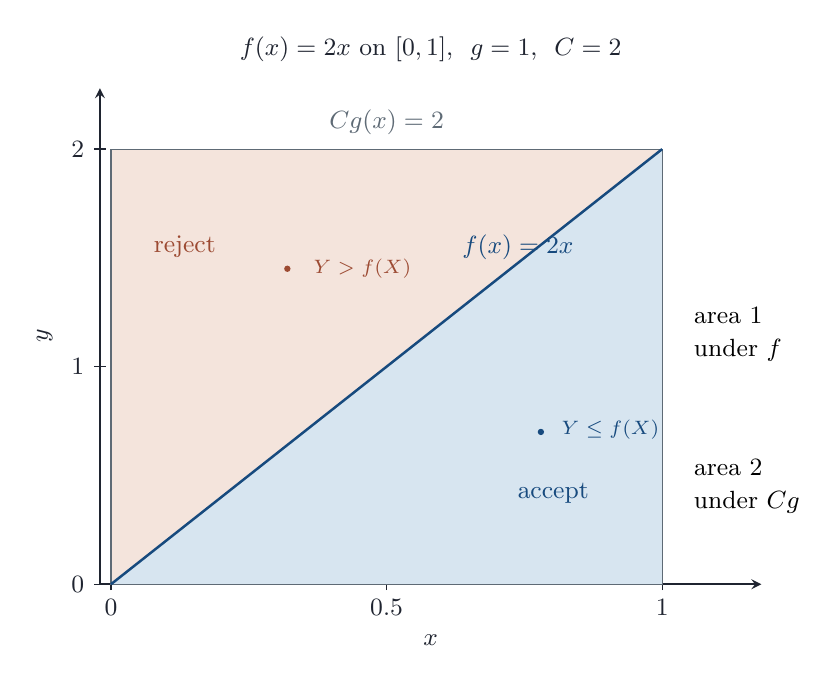
\begin{tikzpicture}
\begin{axis}[
  stat, width=8.4cm, height=6.3cm,
  xmin=-0.02, xmax=1.18, ymin=0, ymax=2.28,
  xtick={0,0.5,1},
  ytick={0,1,2},
  xlabel={$x$},
  ylabel={$y$},
  title={$f(x)=2x$ on $[0,1]$, \ $g=1$, \ $C=2$},
  clip=false,
]
  \fill[accentfill] (axis cs:0,0) rectangle (axis cs:1,2);
  \fill[bluefill] (axis cs:0,0) -- (axis cs:1,0) -- (axis cs:1,2) -- cycle;
  \draw[grey, thin] (axis cs:0,0) rectangle (axis cs:1,2);
  \addplot[statblue, line width=0.9pt, domain=0:1, samples=2] {2*x};
  \node[font=\small, statblue, anchor=west] at (axis cs:0.62,1.55) {$f(x)=2x$};
  \node[font=\small, grey, anchor=south] at (axis cs:0.50,2.02) {$Cg(x)=2$};
  \node[font=\small, accent, anchor=west] at (axis cs:0.06,1.55) {reject};
  \node[font=\small, statblue, anchor=west] at (axis cs:0.72,0.42) {accept};
  \fill[accent] (axis cs:0.32,1.45) circle[radius=1.15pt];
  \fill[statblue] (axis cs:0.78,0.70) circle[radius=1.15pt];
  \node[font=\scriptsize, accent, anchor=west] at (axis cs:0.35,1.45) {$Y>f(X)$};
  \node[font=\scriptsize, statblue, anchor=south west] at (axis cs:0.80,0.62) {$Y\le f(X)$};
  \node[font=\small, anchor=west, align=left] at (axis cs:1.04,1.15)
    {area $1$\\[1pt] under $f$};
  \node[font=\small, anchor=west, align=left] at (axis cs:1.04,0.45)
    {area $2$\\[1pt] under $Cg$};
\end{axis}
\end{tikzpicture}
\end{document}
